\documentclass[11pt, A4paper, norsk]{article}
\usepackage{amsfonts}
\usepackage{amsmath}
\usepackage{amssymb}
\usepackage{amsthm}
\usepackage{babel}
\usepackage{cite}
\usepackage{color}
\usepackage{float}
\usepackage[T1]{fontenc}
\usepackage{graphicx}
\usepackage[colorlinks]{hyperref}
\usepackage[utf8]{inputenc}
\usepackage{listings}
\usepackage{textcomp}


\definecolor{dkgreen}{rgb}{0, 0.6, 0}
\definecolor{gray}{rgb}{0.5, 0.5, 0.5}
\definecolor{daynineyellow}{rgb}{1.0, 0.655, 0.102}
\definecolor{url}{rgb}{0.1, 0.1, 0.4}

\lstset{frame=tb,
	language=csh,
	aboveskip=3mm,
	belowskip=3mm,
	showstringspaces=false,
	columns=flexible,
	basicstyle={\small\ttfamily},
	numbers=none,
	numberstyle=\tiny\color{gray},
	keywordstyle=\color{blue},
	commentstyle=\color{daynineyellow},
	stringstyle=\color{dkgreen},
	breaklines=true,
	breakatwhitespace=true,
	tabsize=3
}

\lstset{inputpath="C:/Users/Torstein/Documents/skole/USN/IIA1319/Assignment 1/DAQ Simulation Application"}
\graphicspath{{C:/Users/Torstein/Documents/USN/IIA1319/Assignment 1/}}
\hypersetup{colorlinks, urlcolor=url}

\author{Torstein Solheim Ølberg | 263054}
\title{Assignment 1 in IIA1319}



%\lstinputlisting{Filnavn! type kodefil}
%\includegraphics[width=12.6cm, height=8cm]{Filnavn! type png}



\begin{document}
\maketitle
\clearpage

\tableofcontents
\clearpage

	\section{Introduction}
		\subsection{Background}
The testing of data manipulation software using datasets from sensors is an important and useful task, but can often become a costly affair if multiple expensive sensors are needed. As a result, the creation of a program capable of simulating multiple sensors and collecting data from them. This Data AcQuisition simulation program would sample sensors at an interval and save the data for later use. The exact parameters for program is decided by the SCE1306DaqCoding application, supplied by Nils-Olav Skeie at \url{https://usn.instructure.com/courses/31275/files/3251058/download?wrap=1}, as shown in figure \ref{params}.
			\begin{figure}
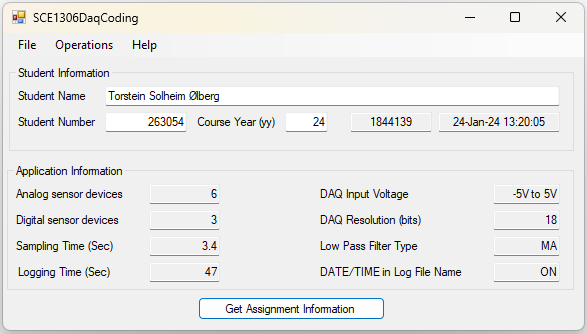
\includegraphics[width=13cm, height=8cm]{parameters.png}
\caption{Screenshot of the SCE1309DaqCoding application with parameters used for the project.}
\label{params}
			\end{figure}
		
				\subsection{Report Structure}
This report contains a description of the resulting program developed, a discussion of the result and a summary of the report. Finally, there are two appendixes. The first appendix is a collection of the documentation for program. The second is a list of the programs developed by an author, and not auto generated by the IDE.
		
		\subsection{Method}
To develop the DAQ simulation program the C\# programming language is used to write the logic and handle user input. As an integrated development environment, Microsoft Visual Studio is used with the inbuilt tools for a Windows Forms Application. Git is used as the version control system, and the repository is uploaded to GitHub. \\
First the development of the GUI front is made. The main view with four buttons, two for logging and two for sampling, and four textboxes for displaying and inputting info. Alongside these are labels, explaining the textboxes purpose, and a menu-strip with a help page option. Then, a sensor class capable of storing a cumulative number and drawing new random number within a range is created. This class is used to set up six sensor instances and produce new samples when needed. Furthermore, a data class is created, capable of storing the samples of six sensors and the date of when they where taken. Also, the handlers for clicking the different buttons and the menu-strip help option are created. They either start a sampling or logging session, sample or log once, or display a message box with info on the app. Then a method each for performing the sampling, extracting the sensor values and saving them to a list of sensor value data classes, and logging, opening a CSV file and writing the data from the data class list into the file. Finally, a pair of timers are added, which keep track of how much time has passed since last logging or sampling was performed and re-enables them as needed.

	\section{Results}
The program created, as seen in figure \ref{ex} consists of a control to start a sampling session, or sample sensors once. The program checks if there has passed a sufficient amount of time since last sampling and either automatically samples again or allows for sampling manually. 
		\begin{figure}
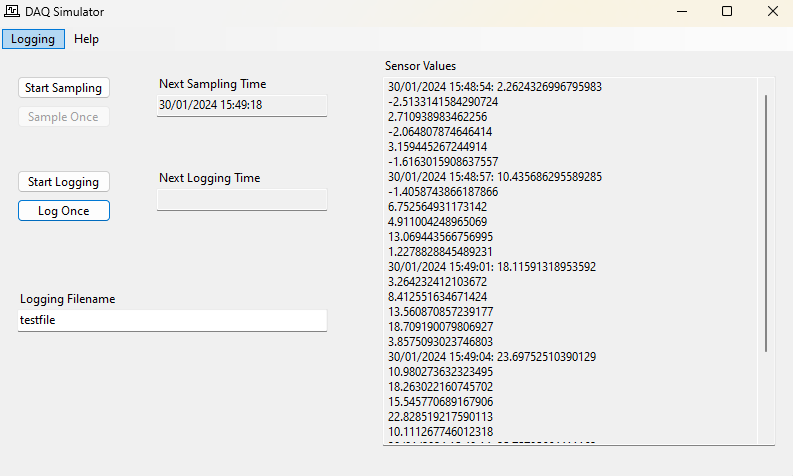
\includegraphics[width=13cm, height=8cm]{Application_Example.png}
\caption{Screenshot of the application during use.}
\label{ex}
		\end{figure}
The same controls are also available for logging, saving all sampled results since last logging was preformed, at a minimum interval of 47 seconds. There is also the option to input a name for the file where the program should log the data. Then there are three windows, two where the time when the next sampling and logging will be available and one where all values whom have been sampled and are reddy to be logged can be viewed. Finally, there is a help page where info on how to use the application can be viewed.
The data logged is saved in a CSV file on the format displayed by this extract:
		\begin{lstlisting}
Date,Sensor 1,Sensor 2,Sensor 3,Sensor 4,Sensor 5,Sensor 6
30/01/2024 15:43:41,2.2624326996795983,-2.5133141584290724,2.710938983462256,-2.064807874646414,3.159445267244914,-1.6163015908637557
		\end{lstlisting}

	\section{Discussion}
The program developed proves that it is possible to create a DAQ program simulating intake from a sensor and saving it in a simple format. However, much more customizability is required for the application to be useful for more than a very specific case. It would be useful to be able to control both the size of the intervals for logging and sampling, as well as the range the sensors pick their random numbers from. It would also be useful for the numbers of sensors used to be changed by the user. Automatic tests for the program to check if it works as expected, and an in-depth analysis of the probability distribution of the random number selector used in this program would also be a good idea, as this will make sure the program functions as expected both now and when further developed. \\
Finally, a low pass filter could be implemented to better simulate analogue data from real sensors, as these can often times have noise which could result in data way out of the normal scope. This filter would be a check of the numbers acquired by the sensor classes and applied to the data before they are stored in the data classes. This would also allow for future real sensors to be used with the application, so as to produce even better testing data.

	\section{Conclusion}
A DAQ simulation program is possible and would be useful to have as an alternative to expensive sensors. This project has produced a simple DAQ application and it can sample and log data from six sensors at intervals. However, this program is very simple and could need a lot more work fro it to be very useful.
	
	\section{Appendix A}
Here you can find the documentation for the program. \\
The program consists of three classes, and an increasing number of objects as a new object is created each time a sampling is performed. However, the base application before any sampling is done consists of 7 objects of these classes.
		\begin{figure}
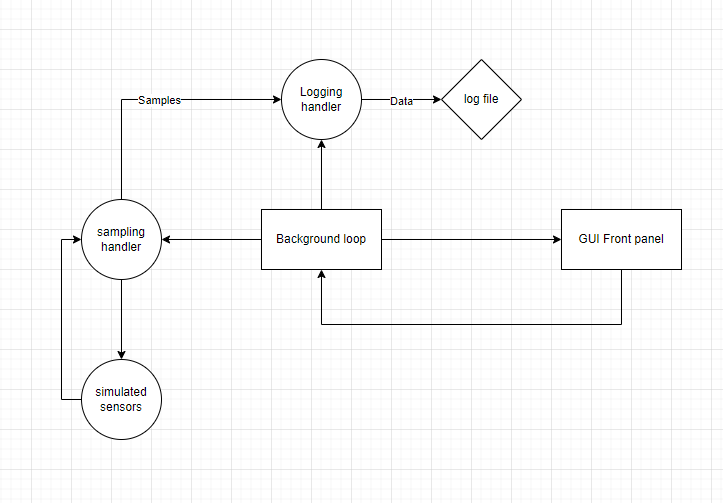
\includegraphics[width=13cm, height=8cm]{Flow_chart.png}
\caption{A flowchart depicting the general structure of the application.}
		\end{figure}
		\begin{figure}
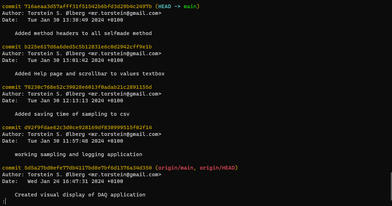
\includegraphics[width=13cm, height=8cm]{git_log.png}
\caption{A list of git commits.}
		\end{figure}
Below follows an example of a log file produced by the program.
\lstinputlisting{data/30_01_2024_15_06_47.csv}

	\section{Appendix B}
Here you can find the code files not made by Visual Studio itself.
\lstinputlisting{Form1.cs}
\lstinputlisting{SensorApp.cs}
\end{document}